%! TEX root = ../main.tex

\subsection{Estado actual}

La enfermería es una profesión técnica, en esta sección se hace una breve reseña
de los métodos de enseñanza fuera del aula que se utilizan actualmente. Se
describe como se realiza la evaluación de los estudiantes, tanto en el área
teórica como en el área práctica. Luego se detallan los principales problemas a
abordar, describiendo los inconvenientes que tiene la metodología actual.

Una observación importante es que la información no bibliográfica presentada en
esta sección, es fruto de reuniones con profesores, encargados y directores de
la carrera de enfermería del \Gls{iab}.

De este modo, se describe el contexto en el que se quiere aplicar una solución.


\subsubsection{Plan de estudio}
\label{sec:plan_estudio}

La carrera de licenciatura en enfermería en el \Gls{iab} tiene una duración de $4$
años, es completamente presencial y tiene una carga total de $3745$
horas. Cada alumno debe aprobar $57$ materias.

Para completar las horas necesarias, las clases se desarrollan en 
dos turnos de manera continua, con excepción de los días donde existen
prácticas de campo. La mayoría de las materias son teóricas, desde segundo curso
acceden a los laboratorios especializados del instituto, y desde el tercer curso
realizan prácticas de campo en hospitales escuela y hospitales con los cuales el
\Gls{iab} tiene convenios.

La carrera cuenta con $150$ alumnos nuevos por año, los mismos se dividen en tres secciones. 
El perfil del egresado de la carrera de licenciatura en enfermería 
es\cite{iab:enfermeria}:

\begin{displayquote}

El profesional egresado de la Licenciatura en Enfermería será capaz de
desempeñar eficientemente el saber teórico y práctico en el campo de su
profesión, valorar las necesidades y problemas bio-psico-sociales y espirituales
del individuo, familia y comunidad, brindando apoyo y proponiendo alternativas
de solución, practicar los valores de honradez, solidaridad y respeto al ser
humano en la prestación de servicios de la salud.

\end{displayquote}

Existen tres formas principales de enseñanza dentro del \Gls{iab}, 
\begin{enumerate*}[label=\itshape\alph*\upshape.]
\item las clases teóricas, 
\item las prácticas de laboratorio y, 
\item las prácticas de campo.
\end{enumerate*}


El plan de estudios se centra en las \emph{competencias básicas} que debe tener
cada alumno al finalizar la materia, estas competencias son facilitadas al
inicio de cada asignatura a los alumnos.

Las competencias básicas son los conocimientos teóricos y prácticos que debe
tener todo profesional de enfermería recién egresado, estas competencias son el
eje central de la carrera y en la obtención de las mismas se centran todas las
actividades curriculares y no curriculares (congresos, encuentros, etc)
realizadas por el \Gls{iab}.



\subsubsection{Prácticas en laboratorios}
\label{sec:practica_lab}

El \Gls{iab} cuenta con un laboratorio especializado para la práctica de los
estudiantes de enfermería. El laboratorio es utilizado por los alumnos 
desde su segundo año de formación, y en el mismo se desarrollan todas las materias 
prácticas, de manera a realizar una formación previa a las prácticas de campo 
explicadas más adelante.

El número de alumnos dificulta la enseñanza individual, por ello las prácticas se
dividen en dos partes, en la primera, similar a una aula tradicional, los
alumnos se sientan y observan al profesor realizar una simulación de
procedimientos sobre un voluntario, en este punto, el profesor realiza las
observaciones que crea son necesarias para llevar a cabo la práctica
profesional, da consejos y responde a las dudas de los alumnos.
Se utilizan modelos del cuerpo humano para simular
algunos procedimientos, en la figura~\ref{fig:iab_veno} se observa un modelo del
brazo humano utilizado para procedimientos de venopunción.

\begin{figure}[h!t] 
\centering 
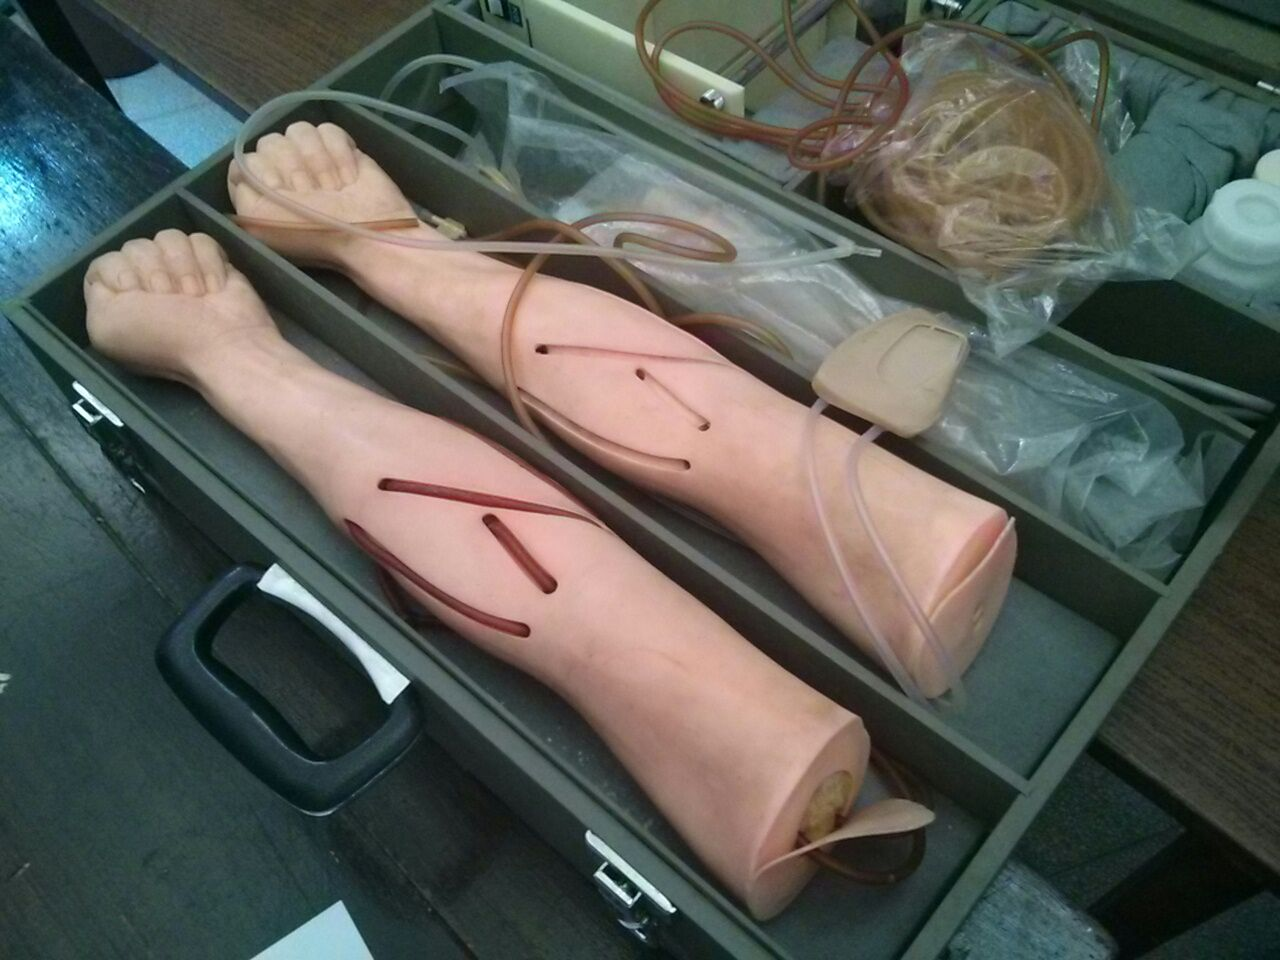
\includegraphics[scale=0.2,natwidth=100,natheight=100]{problema/iab_sala_2.jpg}
\caption{Elementos utilizados para mostrar procedimientos de venopunción}
\label{fig:iab_veno}
\end{figure}

En la segunda parte, los alumnos pasan a un laboratorio que contiene las
herramientas necesarias para la práctica (maniquíes, camas de hospital, y otros
elementos, como se ven en la figura~\ref{fig:iab_lab}), donde pueden explorar y
practicar siempre bajo tutela del profesor. Esto se diferencia
principalmente de la primera parte, en que hay más material para las pruebas y los
alumnos pueden realizar por sí mismos una simulación de los procedimientos.

\begin{figure}[h!t] 
\centering 
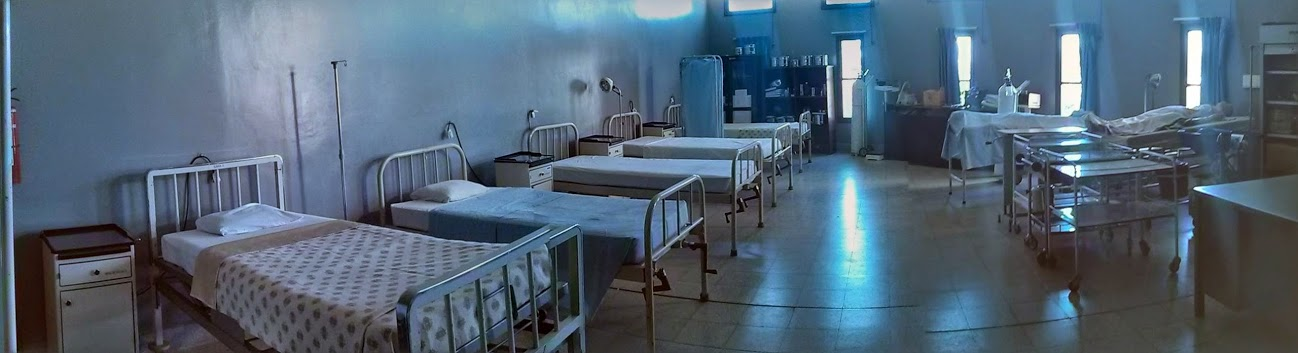
\includegraphics[scale=0.3,natwidth=100,natheight=100]{problema/iab_sala_1.jpg}
\caption{Laboratorio de enfermería del \Gls{iab}}
\label{fig:iab_lab}
\end{figure}


El maniquí que se observa en la figura~\ref{fig:iab_mani}, tiene ciertas
características que facilitan la práctica, por ejemplo, tiene un esquema de los
vasos sanguíneos en ambos brazos. Este maniquí se utiliza además para mostrar
las partes del cuerpo donde se puede realizar la venopunción, para mostrar la
zona específica donde se debe realizar la reanimación, y otras zonas importantes
para la práctica de enfermería.


\begin{figure}[h!t] 
\centering 
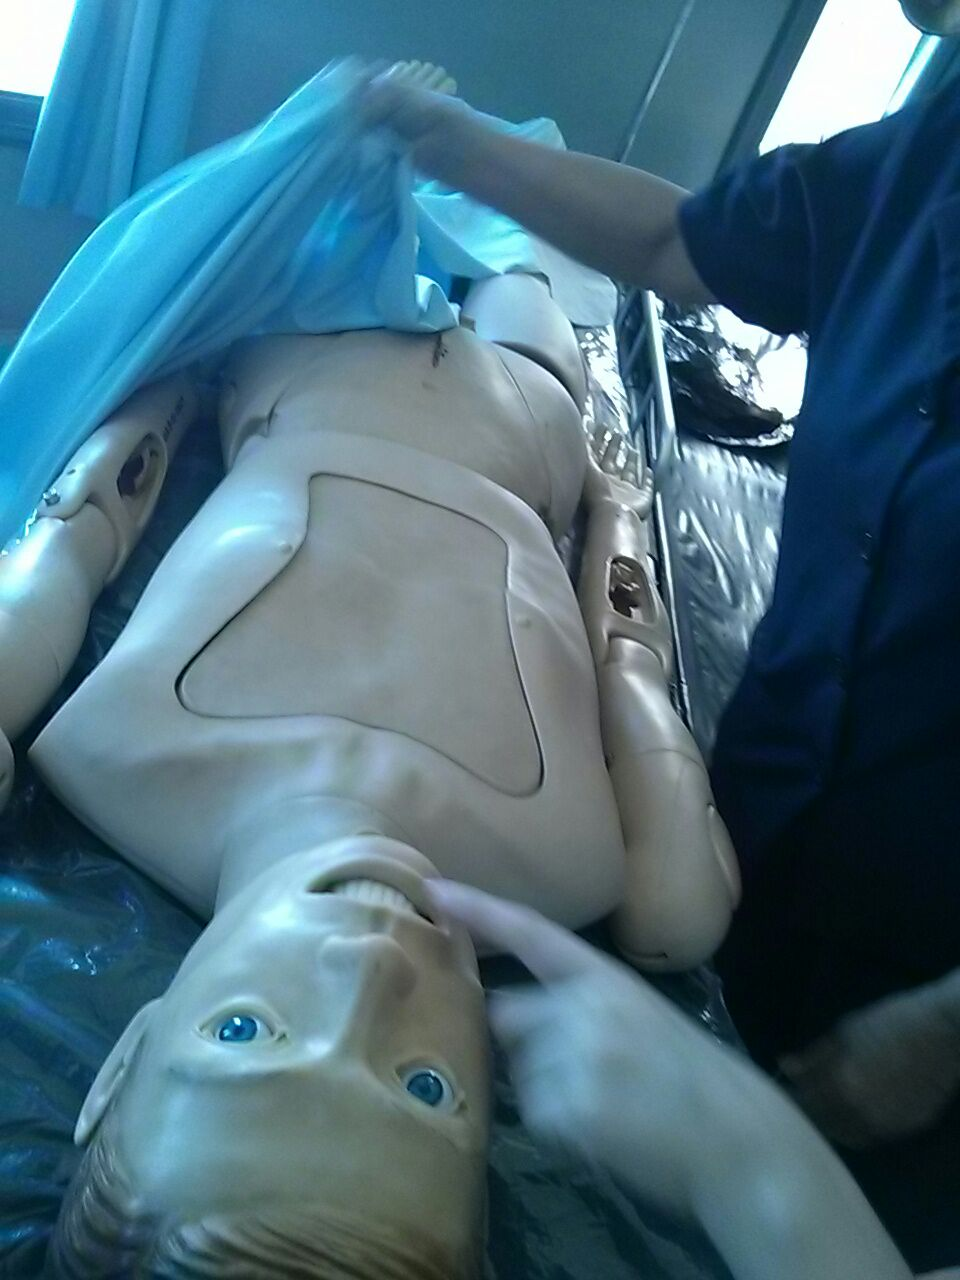
\includegraphics[scale=0.2,natwidth=400,natheight=200]{problema/iab_sala_3.jpg}
\caption{Una instructora de laboratorio muestra las partes del maniquí utilizado
    para en el laboratorio de enfermería.}
\label{fig:iab_mani}
\end{figure}

Además existen varias camas de hospitales (como se observa en la
figura~\ref{fig:iab_lab} a la izquierda), donde se practica la higienización del
paciente, como utilizar los mecanismos de ajuste de la cama, las diferentes
telas utilizadas para las sábanas, y otros aspectos relacionados al cuidado de
un paciente en cama.


\subsubsection{Prácticas de campo}
\label{sec:practica_hos}

Las prácticas de campo son aquellas prácticas profesionales que son
realizadas por los alumnos con pacientes humanos y en hospitales, bajo
supervisión de un profesional y bajo una continua evaluación de sus
acciones, las mismas son llevadas a cabo una vez que los alumnos finalizan
las prácticas de laboratorio.


Los alumnos del \Gls{iab} participan en prácticas de campo 
en diferentes hospitales dependiendo de las necesidades de cada
materia, por ejemplo, los alumnos de \textit{Enfermería en Urgencias} realizan
sus prácticas en el \textit{Centro de Emergencias Médicas}, otros hospitales
utilizados, son el \textit{Hospital de Clínicas}, y diversos hospitales del
\textit{Instituto de Previsión Social}.


Para controlar y medir la evolución de los estudiantes existe un grupo de
profesores cuya función es guiar a los alumnos durante las prácticas de campo,
este grupo de profesores son denominados \textbf{instructores}.

Las prácticas se realizan en grupos que varían de $4$ a $10$ alumnos, dependiendo de
la disponibilidad de instructores y de si el área es crítica o no\footnote{Se
dice que un paciente esta en estado crítico si su vida depende de un
procedimiento externo, como una transfusión de sangre. Un área se considera
crítica si los pacientes en su mayoría son críticos}, un instructor puede
manejar más de un grupo en diferentes horarios. 

Cada instructor posee un planilla por alumno donde se realiza el seguimiento de
sus actividades. La creación de esta planilla de actividades es responsabilidad
del instructor, el instructor debe basarse en las competencias básicas de la
asignatura y la misma es validada por la dirección de la carrera, se considera
que un alumno ha adquirido la pericia\footnote{Sabiduría, práctica, experiencia y 
habilidad en una ciencia o arte.} necesaria para una asignatura solo si pudo
completar la planilla del instructor. Son registradas todas
las actividades del alumno, pero sólo son tomadas en cuenta para el progreso final 
aquellas que son realizadas con la pericia requerida.

\subsubsection{Evaluación a los estudiantes}
\label{sec:problema_evaluacion}

Como dicta su perfil, un egresado de Licenciatura en Enfermería 
debe ser capaz de desempeñar eficientemente su
profesión, el mecanismo que se utiliza para garantizar esto son las
evaluaciones.

Una evaluación es un proceso que permite verificar el grado del progreso del
estudiante en el logro de los objetivos propuestos en cada
asignatura\cite{iab:est_enfemeria}, existen tres tipos de evaluaciones, exámenes
parciales, exámenes finales y evaluación de la práctica de campo.

% VER PARA BORRAR
La cantidad de evaluaciones parciales\footnote{Se
    define examen parcial aquel que mide el rendimiento del período
    correspondiente\cite{iab:est_enfemeria}} está determinada por la materia y el
consenso de los profesores titulares\cite{iab:est_enfemeria}. En cuanto a las 
evaluaciones finales, existen tres períodos en los cuales un alumno puede rendir 
el examen final.


Cada alumno necesita de un $75\%$ de asistencia presencial para tener derecho a
las evaluaciones, así mismo, cada alumno requiere como mínimo $80\%$ de la carga
horaria en prácticas profesionales, el $20\%$ restante lo debe cumplir en un
periodo establecido por el \Gls{iab}.
% esto del 20% restante se puede borrar

En cuanto a la evaluación de la práctica de campo, el enfoque es
subjetivo, es decir depende exclusivamente del instructor de la práctica
determinar si un alumno cuenta o no con la pericia necesaria.
    
Cabe destacar que, si el alumno no aprueba sus prácticas de campo no tiene 
derecho al examen teórico de la materia en cuestión y por lo tanto debe volver 
a cursar la materia. De esta forma, aprobar la práctica de campo se convierte 
en un requisito importante para el progreso del alumno en su vida académica.

El objetivo final de estas evaluaciones es el de evaluar si un alumno comprende
y tiene la pericia necesaria en todas las competencias básicas de una
asignatura.



\subsection{Problemas actuales}
\label{sec:problemas_actuales}
%\observacion{Quizás convenga restar más, tipo sección 4.2}

Si bien el nivel actual de los egresados del \Gls{iab} en la carrera
Licenciatura en Enfermería es satisfactorio, existen ciertos inconvenientes, los
mismos son recabados de distintas fuentes, como tesis de
alumnos\cite{iab:tesis_atencion,iab:tesis_alumnos} y apreciaciones de los
profesores y de alumnos egresados.

En algunos casos los profesores de campo prefieren tener las primeras clases en
el laboratorio antes de ir a los hospitales debido a que se suelen presentar los
siguientes inconvenientes:

\begin{itemize}

    \item \textbf{Falta de preparación de los alumnos:} ciertos detalles
        necesarios para la práctica de campo no son completamente cubiertos en
        el laboratorio.

    \item \textbf{Nerviosismo ante primera práctica:} ciertos alumnos reaccionan
        de manera inesperada la primera vez que deben realizar una práctica,
        esto se debe principalmente a que ciertos procedimientos son impactantes
        y ni el laboratorio ni el aula pueden preparar para este tipo de
        experiencias.
                
    \item \textbf{Definición de un protocolo de comunicación:} en la práctica de
        campo, los profesores necesitan comunicarse con sus alumnos de una
        manera rápida y eficiente, debido a esto los profesores enseñan a sus
        alumnos ciertos códigos que son utilizados para corregir, notificar y
        enseñar durante la práctica.
          
\end{itemize}


En cuanto al punto de vista de los alumnos, los principales inconvenientes que
tienen los alumnos de enfermería del \Gls{iab} son:

\begin{itemize}

    \item \textbf{Carga horaria de trabajos prácticos:} se refiere al tiempo
        necesario por los estudiantes para llevar a cabo un trabajo
        práctico\cite{iab:tesis_alumnos}.
        
    \item \textbf{Carga horaria de materias teóricas:} se refiere al tiempo que
        consumen las materias teóricas, cuyo tiempo de estudio es reducido por
        la necesidad de acudir a prácticas de campo en horarios
        variados\cite{iab:tesis_alumnos}.
        

    \item \textbf{Falta de materiales para los profesores:} la enfermería es un
        área en constante evolución, los materiales se vuelven obsoletos
        rápidamente, y los profesores no cuentan con una fuente actualizada de
        información\cite{iab:tesis_alumnos}.
        
    \item \textbf{Problemas de transporte:} la ubicación del \Gls{iab} facilita
        el acceso al mismo desde rutas internacionales, pero no se puede decir
        lo mismo de los hospitales donde se realizan prácticas
        profesionales\cite{iab:tesis_alumnos}. 
        
        Este problema es acentuado por la gran cantidad de tiempo que deben
        pasar los alumnos en los medios de transporte para moverse desde sus
        respectivos hogares hasta el \Gls{iab} o a los campos de
        práctica\cite{iab:tesis_alumnos}.
        
        Adicionalmente, la población del \Gls{iab} esta compuesta en su gran
        mayoría por personas de niveles económicos medio-bajos y un gran
        porcentaje de los alumnos son del interior del
        país\cite{iab:tesis_alumnos}.
    
    \item \textbf{Preparación para las prácticas:} los alumnos rara vez están
        completamente preparados la primera vez que realizan una práctica de
        campo, muchos sufren ataques de pánico y no pueden reaccionar de manera
        correcta.
        
    \item \textbf{Cantidad de alumnos:} debido a la cantidad de alumnos, las
        prácticas de campo rara vez se realizan en un sólo hospital, para
        asignaturas críticas, se forman aproximadamente $35$ grupos de
        estudiantes.

\end{itemize}
